% !Mode:: "TeX:UTF-8"
\documentclass{article}

%%%%%%%%------------------------------------------------------------------------
%%%% 日常所用宏包

%% 控制页边距
% 如果是beamer文档类, 则不用geometry
\makeatletter
\@ifclassloaded{beamer}{}{\usepackage[top=2.5cm, bottom=2.5cm, left=2.5cm, right=2.5cm]{geometry}}
\makeatother

%% 控制项目列表
\usepackage{enumerate}

%% 多栏显示
\usepackage{multicol}

%% 算法环境
\usepackage{algorithm}  
\usepackage{algorithmic} 
\usepackage{float} 

%% 网址引用
\usepackage{url}

%% 控制矩阵行距
\renewcommand\arraystretch{1.4}

%% hyperref宏包,生成可定位点击的超链接,并且会生成pdf书签
\makeatletter
\@ifclassloaded{beamer}{
\usepackage{hyperref}
}{
\usepackage[%
    pdfstartview=FitH,%
    CJKbookmarks=true,%
    bookmarks=true,%
    bookmarksnumbered=true,%
    bookmarksopen=true,%
    colorlinks=true,%
    citecolor=blue,%
    linkcolor=blue,%
    anchorcolor=green,%
    urlcolor=blue%
]{hyperref}
}
\makeatother



\makeatletter % 如果是 beamer 不需要下面两个包
\@ifclassloaded{beamer}{

}{
%% 控制标题
\usepackage{titlesec}
%% 控制目录
\usepackage{titletoc}
}
\makeatother

%% 控制表格样式
\usepackage{booktabs}

%% 控制字体大小
\usepackage{type1cm}

%% 首行缩进,用\noindent取消某段缩进
\usepackage{indentfirst}

%% 支持彩色文本、底色、文本框等
\usepackage{color,xcolor}

%% AMS LaTeX宏包: http://zzg34b.w3.c361.com/package/maths.htm#amssymb
\usepackage{amsmath,amssymb}

%%%% 基本插图方法
%% 图形宏包
\usepackage{graphicx}

%% 多个图形并排
\usepackage{subfig}

%%%% 基本插图方法结束

%%%% pgf/tikz绘图宏包设置
\usepackage{pgf,tikz}
\usetikzlibrary{shapes,automata,snakes,backgrounds,arrows}
\usetikzlibrary{mindmap}
%% 可以直接在latex文档中使用graphviz/dot语言,
%% 也可以用dot2tex工具将dot文件转换成tex文件再include进来
%% \usepackage[shell,pgf,outputdir={docgraphs/}]{dot2texi}
%%%% pgf/tikz设置结束


\makeatletter % 如果是 beamer 不需要下面两个包
\@ifclassloaded{beamer}{

}{
%%%% fancyhdr设置页眉页脚
%% 页眉页脚宏包
\usepackage{fancyhdr}
%% 页眉页脚风格
\pagestyle{plain}
}

%% 有时会出现\headheight too small的warning
\setlength{\headheight}{15pt}

%% 清空当前页眉页脚的默认设置
%\fancyhf{}
%%%% fancyhdr设置结束


\makeatletter % 对 beamer 要重新设置
\@ifclassloaded{beamer}{

}{
%%%% 设置listings宏包用来粘贴源代码
%% 方便粘贴源代码,部分代码高亮功能
\usepackage{listings}

%% 设置listings宏包的一些全局样式
%% 参考http://hi.baidu.com/shawpinlee/blog/item/9ec431cbae28e41cbe09e6e4.html
\lstset{
showstringspaces=false,              %% 设定是否显示代码之间的空格符号
numbers=left,                        %% 在左边显示行号
numberstyle=\tiny,                   %% 设定行号字体的大小
basicstyle=\footnotesize,                    %% 设定字体大小\tiny, \small, \Large等等
keywordstyle=\color{blue!70}, commentstyle=\color{red!50!green!50!blue!50},
                                     %% 关键字高亮
frame=shadowbox,                     %% 给代码加框
rulesepcolor=\color{red!20!green!20!blue!20},
escapechar=`,                        %% 中文逃逸字符,用于中英混排
xleftmargin=2em,xrightmargin=2em, aboveskip=1em,
breaklines,                          %% 这条命令可以让LaTeX自动将长的代码行换行排版
extendedchars=false                  %% 这一条命令可以解决代码跨页时,章节标题,页眉等汉字不显示的问题
}}
\makeatother
%%%% listings宏包设置结束


%%%% 附录设置
\makeatletter % 对 beamer 要重新设置
\@ifclassloaded{beamer}{

}{
\usepackage[title,titletoc,header]{appendix}
}
\makeatother
%%%% 附录设置结束


%%%% 日常宏包设置结束
%%%%%%%%------------------------------------------------------------------------


%%%%%%%%------------------------------------------------------------------------
%%%% 英文字体设置结束
%% 这里可以加入自己的英文字体设置
%%%%%%%%------------------------------------------------------------------------

%%%%%%%%------------------------------------------------------------------------
%%%% 设置常用字体字号,与MS Word相对应

%% 一号, 1.4倍行距
\newcommand{\yihao}{\fontsize{26pt}{36pt}\selectfont}
%% 二号, 1.25倍行距
\newcommand{\erhao}{\fontsize{22pt}{28pt}\selectfont}
%% 小二, 单倍行距
\newcommand{\xiaoer}{\fontsize{18pt}{18pt}\selectfont}
%% 三号, 1.5倍行距
\newcommand{\sanhao}{\fontsize{16pt}{24pt}\selectfont}
%% 小三, 1.5倍行距
\newcommand{\xiaosan}{\fontsize{15pt}{22pt}\selectfont}
%% 四号, 1.5倍行距
\newcommand{\sihao}{\fontsize{14pt}{21pt}\selectfont}
%% 半四, 1.5倍行距
\newcommand{\bansi}{\fontsize{13pt}{19.5pt}\selectfont}
%% 小四, 1.5倍行距
\newcommand{\xiaosi}{\fontsize{12pt}{18pt}\selectfont}
%% 大五, 单倍行距
\newcommand{\dawu}{\fontsize{11pt}{11pt}\selectfont}
%% 五号, 单倍行距
\newcommand{\wuhao}{\fontsize{10.5pt}{10.5pt}\selectfont}
%%%%%%%%------------------------------------------------------------------------


%% 设定段间距
\setlength{\parskip}{0.5\baselineskip}

%% 设定行距
\linespread{1}


%% 设定正文字体大小
% \renewcommand{\normalsize}{\sihao}

%制作水印
\RequirePackage{draftcopy}
\draftcopyName{XTUMESH}{100}
\draftcopySetGrey{0.90}
\draftcopyPageTransform{40 rotate}
\draftcopyPageX{350}
\draftcopyPageY{80}

%%%% 个性设置结束
%%%%%%%%------------------------------------------------------------------------


%%%%%%%%------------------------------------------------------------------------
%%%% bibtex设置

%% 设定参考文献显示风格
% 下面是几种常见的样式
% * plain: 按字母的顺序排列,比较次序为作者、年度和标题
% * unsrt: 样式同plain,只是按照引用的先后排序
% * alpha: 用作者名首字母+年份后两位作标号,以字母顺序排序
% * abbrv: 类似plain,将月份全拼改为缩写,更显紧凑
% * apalike: 美国心理学学会期刊样式, 引用样式 [Tailper and Zang, 2006]

\makeatletter
\@ifclassloaded{beamer}{
\bibliographystyle{apalike}
}{
\bibliographystyle{unsrt}
}
\makeatother


%%%% bibtex设置结束
%%%%%%%%------------------------------------------------------------------------

%%%%%%%%------------------------------------------------------------------------
%%%% xeCJK相关宏包

\usepackage{xltxtra,fontspec,xunicode}
\usepackage[slantfont, boldfont]{xeCJK} 

%% 针对中文进行断行
\XeTeXlinebreaklocale "zh"             

%% 给予TeX断行一定自由度
\XeTeXlinebreakskip = 0pt plus 1pt minus 0.1pt

%%%% xeCJK设置结束                                       
%%%%%%%%------------------------------------------------------------------------

%%%%%%%%------------------------------------------------------------------------
%%%% xeCJK字体设置

%% 设置中文标点样式,支持quanjiao、banjiao、kaiming等多种方式
\punctstyle{kaiming}                                        
                                                     
%% 设置缺省中文字体
\setCJKmainfont[BoldFont={Adobe Heiti Std}, ItalicFont={Adobe Kaiti Std}]{Adobe Song Std}   
%% 设置中文无衬线字体
\setCJKsansfont[BoldFont={Adobe Heiti Std}]{Adobe Kaiti Std}  
%% 设置等宽字体
\setCJKmonofont{Adobe Heiti Std}                            

%% 英文衬线字体
\setmainfont{DejaVu Serif}                                  
%% 英文等宽字体
\setmonofont{DejaVu Sans Mono}                              
%% 英文无衬线字体
\setsansfont{DejaVu Sans}                                   

%% 定义新字体
\setCJKfamilyfont{song}{Adobe Song Std}                     
\setCJKfamilyfont{kai}{Adobe Kaiti Std}
\setCJKfamilyfont{hei}{Adobe Heiti Std}
\setCJKfamilyfont{fangsong}{Adobe Fangsong Std}
\setCJKfamilyfont{lisu}{LiSu}
\setCJKfamilyfont{youyuan}{YouYuan}

%% 自定义宋体
\newcommand{\song}{\CJKfamily{song}}                       
%% 自定义楷体
\newcommand{\kai}{\CJKfamily{kai}}                         
%% 自定义黑体
\newcommand{\hei}{\CJKfamily{hei}}                         
%% 自定义仿宋体
\newcommand{\fangsong}{\CJKfamily{fangsong}}               
%% 自定义隶书
\newcommand{\lisu}{\CJKfamily{lisu}}                       
%% 自定义幼圆
\newcommand{\youyuan}{\CJKfamily{youyuan}}                 

%%%% xeCJK字体设置结束
%%%%%%%%------------------------------------------------------------------------

%%%%%%%%------------------------------------------------------------------------
%%%% 一些关于中文文档的重定义
\newcommand{\chntoday}{\number\year\,年\,\number\month\,月\,\number\day\,日}
%% 数学公式定理的重定义

%% 中文破折号,据说来自清华模板
\newcommand{\pozhehao}{\kern0.3ex\rule[0.8ex]{2em}{0.1ex}\kern0.3ex}

\newtheorem{example}{例}                                   
\newtheorem{theorem}{定理}[section]                         
\newtheorem{definition}{定义}
\newtheorem{axiom}{公理}
\newtheorem{property}{性质}
\newtheorem{proposition}{命题}
\newtheorem{lemma}{引理}
\newtheorem{corollary}{推论}
\newtheorem{remark}{注解}
\newtheorem{condition}{条件}
\newtheorem{conclusion}{结论}
\newtheorem{assumption}{假设}

\makeatletter %
\@ifclassloaded{beamer}{

}{
%% 章节等名称重定义
\renewcommand{\contentsname}{目录}     
\renewcommand{\indexname}{索引}
\renewcommand{\listfigurename}{插图目录}
\renewcommand{\listtablename}{表格目录}
\renewcommand{\appendixname}{附录}
\renewcommand{\appendixpagename}{附录}
\renewcommand{\appendixtocname}{附录}
%% 设置chapter、section与subsection的格式
\titleformat{\chapter}{\centering\huge}{第\thechapter{}章}{1em}{\textbf}
\titleformat{\section}{\centering\sihao}{\thesection}{1em}{\textbf}
\titleformat{\subsection}{\xiaosi}{\thesubsection}{1em}{\textbf}
\titleformat{\subsubsection}{\xiaosi}{\thesubsubsection}{1em}{\textbf}

\@ifclassloaded{book}{

}{
\renewcommand{\abstractname}{摘要}
}
}
\makeatother

\renewcommand{\figurename}{图}
\renewcommand{\tablename}{表}

\makeatletter
\@ifclassloaded{book}{
\renewcommand{\bibname}{参考文献}
}{
\renewcommand{\refname}{参考文献} 
}
\makeatother

\floatname{algorithm}{算法}
\renewcommand{\algorithmicrequire}{\textbf{输入:}}
\renewcommand{\algorithmicensure}{\textbf{输出:}}

%%%% 中文重定义结束
%%%%%%%%------------------------------------------------------------------------

\setCJKmainfont{STKaiti} % 如果请替换为本地系统有的字体
%中文断行
\XeTeXlinebreaklocale "zh"
\XeTeXlinebreakskip = 0pt plus 1pt minus 0.1pt
\newcommand{\Span}{\text{span}}
\newcommand{\Null}{\text{Null}}
\newcommand{\Ran}{\text{Ran}}
\begin{document}
\title{第一章$\qquad$线性代数的背景}
%\date{\today}
\maketitle  %定义时间和标题
%\tableofcontents
%\newpage
\section{}
\subsection{矩阵}
在这一章中,向量空间是定义在复数域上的,$\mathrm{C}^{n\times m}$ 表示由所有定义在$C$上的$n\times m$的矩阵构成的向量空间。

加法:$C=A+B$,这里的$A$,$B$和$C$都$\in\mathrm{C}^{n\times m}$,即$c_{ij}=a_{ij}+b_{ij}$.

数乘:$C=\alpha A$,即$c_{ij}=\alpha a_{ij}$.

乘法:$C=AB$,这里A$\in\mathrm{C}^{n\times m}$,B$\in\mathrm{C}^{m\times p}$,C$\in\mathrm{C}^{n\times p}$,即$c_{ij}=\sum_{k=1}^m a_{ik}b_{kj}$.

$a_{*j}$表示矩阵A的第j列,$a_{i*}$表示矩阵A的第i行.
$A^H$表示矩阵$A$的转置共轭矩阵,即$A^H=\bar{A}^H=\bar{A^T}$.
\subsection{方阵与特征值}






$I$表示单位矩阵,若$CA=AC=I$,则称矩阵$C$为矩阵$A$的逆矩阵$A^{-1}$.

$det(A)=a_{11}A_{11}-a_{12}A_{11}+\cdots+(-1)^{1+n}a_{1n}A_{1n}=\sum_{j=1}^n (-1)^{j+1} a_{1j}det(A_{1j}) .$  

如果$det(A)=0$,则称矩阵$A$是奇异的,否则称$A$为非奇异的.

$$det(AB)=det(A)det(B),$$

$$det(A^T)=det(A),$$

$$det(\alpha A)=\alpha ^n det(A),$$

$$det(\bar{A})=\overline{det(A)},$$

$$det(I)=1.$

\newtheorem{definition}{定义}
\begin{definition}
设$A$是$n$阶方阵,如果存在数$\lambda$和非零$n$维列向量$u$,使得$Au=\lambda u$成立,则称$\lambda$是$A$的一个特征值,非零向量$u$称为矩阵$A$的对应于特征值$\lambda$的特征向量.

$p_A(\lambda)=det(A-\lambda I)$称为矩阵$A$的特征多项式,$\lambda $是矩阵$A$的特征值当且仅当
$$det(A-\lambda I)\equiv p_A(\lambda)=0,$$
即$\lambda$是矩阵$A$的特征多项式的一个根.

矩阵$A$的谱是指$A$的所有特征值组成的集合,记为$\sigma (A)$.

矩阵$A$是奇异的当且仅当$A$有一个特征值为$0$.
\end{definition}

\newtheorem{proposition}{命题}
\begin{proposition}
矩阵$A$是非奇异的当且仅当$A$可逆.

矩阵$A$的谱半径等于矩阵$A$的特征值的模的最大值,记为$\rho (A)$,矩阵$A$的迹等于$A$的所有对角线元素的和,记为$tr(A)=\sum_{i=1}^n a_{ii}$,也等于$A$的所有特征值的和.
\end{proposition}

\newtheorem{proposition}{命题}
\begin{proposition}
如果$\lambda$是矩阵$A$的特征值,那么$\bar\lambda$是矩阵$A^H$的特征值。

如果存在一个非零列向量$x$使得$Ax=\lambda x$,则称$\lambda $为一个右特征值,$x$称为矩阵$A$的特征值$\lambda $的右特征向量.
如果存在一个非零列向量$y$使得$yA=y\lambda$,则称$\lambda $为一个左特征值,$y$称为矩阵$A$的特征值$\lambda $的左特征向量.

$$Au=\lambda u,v^HA=\lambda v^H.$$

$$u^HA^H=\bar{\lambda}u^H,A^Hv=\bar{\lambda}v.$$
\end{proposition}

\subsection{矩阵类型}
接下来介绍一些特殊的矩阵类型:

\begin{tabular}{ |l|l| }   
\hline   
矩阵类型 & 含义\\
\hline
对称矩阵 & $A^T=A$ \\
\hline
Hermitian矩阵 & $A^H=A$ \\
\hline
反对称矩阵 & $A^T=-A$ \\
\hline
反埃尔米特矩阵 &  $A^H=-A$ \\
\hline
正规矩阵 &  $A^HA=AA^H$ \\
\hline
非负矩阵 & $a_{j}\ge 0,i,j=1,...,n$(同理定义非正矩阵) \\
\hline
酉矩阵 & $Q^HQ=I$ \\
\hline 
对角矩阵 & $a_{ij}=0,i\neq j$,记$A=diag(a_{11},a_{22},...,a_{nn})$ \\
\hline
上三角矩阵 & $a_{ij}=0,i>j$,类似,下三角矩阵:$a_{ij}=0,i<j$ \\
\hline
上双对角线矩阵 & $a_{ij}=0,i\neq j$,或者$j\neq i+1$.类似,下双对角矩阵:$a_{ij}=0,i\neq j$,或者$j\neq i-1$ \\
\hline 
三对角线矩阵 & $a_{ij}=0,|j-i|>1$,形如$A=tridiag(a_{i,i-1},a_{ii},a_{i,i+1})$ \\
\hline
带矩阵 & $a_{ij}\neq 0,i-m_l\leqslant j\leqslant i+m_u$,$m_l,m_u$是两个非负整数,数$m_l+m_u+1$叫做矩阵的带宽 \\
\hline
Upper Hessenberg 矩阵 & $a_{ij}=0,i>j+1$.类似 Lower Hessenberg矩阵:$a_{ij}=0,i<j-1$ \\
\hline 
外积矩阵 & $A=uv^H$,此处的$uv$为列向量 \\
\hline
置换矩阵 &它在每行和每列中只有一个$1$,而在其他地方则为$0$ \\
\hline
分块对角矩阵 & $A$的分块矩阵只有在主对角线上有非零子块,其余子块都为零矩阵,且非零子块都是方阵 \\
\hline
块三对角矩阵 & 非零系数在如下的三条对角线上:主对角线、低对角线、高对角线 \\
\hline
\end{tabular}


\subsection{向量内积和范数}
在一个向量空间$X$中,内积是一个$X\times X$到R(C)的一个映射:$x\epsilon X,y\epsilon X \longrightarrow s(x,y)\epsilon R $,且它满足如下条件:

1.$s(x,y)$是关于$x$是线性的,$s(\lambda _1 x_1+\lambda _2 x_2)=\lambda _1 s(x_1,y)+\lambda _2 s(x_2,y),\forall x,y\epsilon X,\forall \lambda _1 ,\lambda _2 \epsilon R(C)$.

2.$s(x,y)=\overline{s(y,x)},\forall x,y\epsilon X$,当$x,y$取实数域时$s(x,y)=s(y,x)$.

3.$s(x,y)\ge 0$当且仅当$x=0$时,等号成立.

4.Cauchy-Schwartz不等式:$(\vert s(x,x)\vert)^2\leqslant s(x,x)s(y,y)$.

特别注意当X空间取复数域时,内积$(x,y)=\sum_{i=1}^n x_i\bar{y}_i$,它经常被写成$(x,y)=y^Hx$.欧几里德内积在矩阵计算中的一个基本性质:$(Ax,y)=(x,A^Hy),\forall x,y\epsilon C$.

\newtheorem{proposition}{命题}
\begin{proposition}
酉矩阵对向量作用后的内积是欧几里德内积,$(Qx,Qy)=(x,y)$,对任意酉矩阵和向量$x,y$都成立.
\end{proposition}

证明:$(Qx,Qy)=(x,Q^HQ)=(x,y)$.

在内积空间中,我们可以定义范数,令$\parallel x\parallel=\sqrt{(x,x)}$,则此由内积定义的范数满足:

1.$\parallel x\parallel \ge 0,\forall x\epsilon X$,并且$\parallel x\parallel=0$当且仅当$x=0$.

2.$\parallel \alpha x\parallel =|\alpha| \parallel x\parallel,\forall x\epsilon X,\forall \alpha \epsilon C$.

3.$\parallel x+y \parallel \leqslant \parallel x\parallel + \parallel y\parallel ,\forall x,y\epsilon X$.

从上面的命题可以看出,一个酉矩阵作用向量后是保范的,$\parallel Qx \parallel_2=\parallel x \parallel_2,\forall ~x$.由此我们可以看出酉矩阵是保范的.下面介绍向量的几个范数:
$\parallel x \parallel_p=(\sum_{i=1}^n |x_i|^p)^{1/p}$.且当$p=1,2,\infty$时

$$\parallel x \parallel_1=|x_1|+|x_2|+...+|x_n|,$$

$$\parallel x \parallel_2=[|x_1|^2+|x_2|^2+..+|x_n|^2]^{1/2},$$

$$\parallel x \parallel_\infty=\max |x_i|,$$

Cauchy-Schwartz不等式变成$|(x,y)|\leqslant \parallel x \parallel_2\parallel y\parallel_2$.

\subsection{矩阵范数}

设矩阵A$\in\mathrm{C}^{n\times m}$,定义矩阵$A$的范数
$$\parallel A\parallel _{pq}=max\frac{\parallel Ax\parallel _p}{\parallel x\parallel _q},$$
这里$x\neq 0$,$x\in\mathrm{C}^{m}$.

范数满足下面的性质:

$$\parallel A\parallel\ge 0,\forall A\in\mathrm{C}^{n\times m},$$并且$\parallel A\parallel = 0$当且仅当$A=0$.

$$\parallel\alpha A\parallel = |\alpha|\parallel A\parallel,\forall A\in\mathrm{C}^{n\times m},\forall\alpha\in\mathrm{C}.$$

$$\parallel A+B\parallel\leqslant\parallel A\parallel+\parallel B\parallel,\forall A,B\in\mathrm{C}^{n\times m}.$$

当$q=p$时的范数称为p-范数,有
$$\parallel AB\parallel _p\leqslant\parallel A\parallel _p\parallel B\parallel_p.$$

对于方阵$A$,有$\parallel A^k\parallel_p\leqslant\parallel A\parallel ^k _p$,如果$A^k$的$p-$范数小于1,那么$A^k$收敛到0。

矩阵$A$的Frobenius范数定义为$(\sum_{j=1}^m\sum_{i=1}^n |a_{ij}|^2)^{1/2}$.

$\parallel A\parallel_1 = max\sum_{i=1}^n |a_{ij}|$,j=1,2,$\cdots$,m.

$\parallel A\parallel_\infty= max\sum_{j=1}^m |a_{ij}|$,i=1,2,$\cdots$,n.

$\parallel A\parallel_2=[\rho(A^HA)]^{1/2}=[\rho(AA^H)]^{1/2}$.

$\parallel A\parallel_F=[tr(A^HA)]^{1/2}=[tr(AA^H)]^{1/2}$.

设A$\in\mathrm{C}^{n\times m}$,$A^HA$的特征值是非负的,令$q=min(n,m)$,$A^HA$的q个非负特征值的算术平方根叫作$A$的奇异值.$\parallel A\parallel_2$等于矩阵$A$的最大的奇异值,记为$\sigma_1$.

\subsection{子空间,秩和核}
向量集$G=\lbrace a_1,a_2,\cdots,a_q\rbrace$的所有线性组合是一个向量子空间,叫做$G$的线性扩张.

%\span\null\ran

$$ \Span G=\Span\lbrace a_1,a_2,\cdots,a_q\rbrace=\lbrace z\in\mathrm{C}^n|z=\sum_{i=1}^q{\alpha _i a_i},\lbrace\alpha _i\rbrace_{i=1,2,\cdots q}\in\mathrm{C}^n\rbrace.$$
如果$a_1,a_2,\cdots,a_q$是线性无关的,那么$a_1,a_2,\cdots,a_q$叫做$ \span{G}$的一组基.

给定两个向量子空间$S_1$和$S_2$,它们的和$S=S_1+S_2$也是一个向量子空间,定义为$S_1$中的所有向量和$S_2$中的所有向量的和。两个向量子空间的交集还是一个子空间,如果交集为${0}$,则称$S_1$与$S_2$的和为直和,记为$S=S_1\bigoplus S_2$.当S等于$C^n$时,$\forall x\in C^n$,存在唯一的向量$x_1\in S_1$和$x_2\in S_2$,使得$x=x_1+x_2$,即分解是唯一的.

矩阵$A$有两个重要的子空间,记为$ \Ran(A)=\lbrace Ax|x\in\mathrm{C}^m\rbrace$;和它的核(零空间),记为$ \Null(A)=\lbrace x\in\mathrm{C}^m|Ax=0\rbrace$.
 
矩阵$A\in\mathrm{C}^{n\times m}$的秩等于线性无关的列数,也等于线性无关的行数;当$A$的秩等于$m$和$n$的最小值时,就说$A$是满秩的.

$$\mathrm{C}^n=\Ran(A)\bigoplus \Null(A^T),\mathrm{C}^m=\Ran(A^T)\bigoplus \Null(A).$$

当$AS\subset S$时,就说子空间$S$在方阵$A$下是不变的,比如$ \Null(A-\lambda I)$在矩阵$A$下是不变的,$ \Null(A-\lambda I)$子空间称为与$\lambda$相关的特征子空间,由矩阵$A$的特征值$\lambda$的所有特征向量再加上零向量构成.


\subsection{正交向量和子空间}
一个向量集合$G=\lbrace a_1,a_2,...a_r\rbrace$如果满足$(a_i,a_j)=0,i\neq j$,则称为正交集.且对$G$的每一个向量$\parallel a_i \parallel_2=1$,称为标准正交集.一个向量正交于子空间$S$的每一个向量,就称正交于这个子空间.与$S$所有正交的向量的构成的集合是一个子空间,称为$S$的正交补,记$S^\perp$.且任何向量都可以分解成$S$与$S^\perp$中的向量和.

每一个子空间都有一个标准正交基,这个标准正交基是通过任意一组基标准正交化得到的,通常用Gram-Schmidt算法求出.

\begin{definition}
设$A\epsilon C^{n\times n}$,如果存在$n$阶酉矩阵$Q$和$n$阶上三角矩阵$R$,使$A=QR$则称之为$A$的$QR$分解或酉三角分解。当$A\epsilon R^{n\times n}$时,称为$A$的正三角分解。
\end{definition}

任意满秩实(复)矩阵$A$,都可以唯一地分解$A=QR$,其中$Q$为正交(酉)矩阵,$R$是具有正对角元的上三角矩阵。
\subsection{矩阵的规范形式}
下面讨论将方阵简化对角线形式,或者上三角形式的简单方阵。且这种简单转化保留特征值不变。

\begin{definition}
矩阵$A,B$称为相似的,如果存在一个非奇异矩阵$X$使得   $A=X^{-1}BX.$  
\end{definition}

对进行运算称为对进行相似变换,称可逆矩阵为相似变换矩阵。

下面介绍一些定义:

1.矩阵$A$的一个特征值的有几重根,这个几重根就叫做这个特征值的代数重数。

2.如果一个特征值的代数重数是1,则这个特征值是简单的;矩阵$A$的特征值代数重数不是1,则是非简单的。

3.矩阵$A$的特征值所对应的特征向量所构成空间(即特征子空间,也是方程组$(λI-A)x=0$的维数,称为几何重数。

4.如果$A$的某个特征值的几何重数严格小于代数重数,我们就说$A$是有亏的;如果$A$的每个特征值的几何重数都与它的代数重数相等,我们就称$A$是无亏的;如果$A$的每个特征值的几何重数都是1,我们称A是无损的,否则有损的。
\subsubsection{矩阵可对角化}
\newtheorem{thm}{定理}
\begin{thm}
$n$维矩阵可对角化,当且仅当它有$n$个线性无关的特征向量。
\end{thm}

\newtheorem{thm}{定理}
\begin{thm}
$n$维矩阵可对角化,当且仅当它的所有特征值是半单特征值。(半单特征值指特征值无重根)
\end{thm}

\subsubsection{若尔当标准型}
\begin{definition}
若尔当标准型是由若干个主对角线为特征值,下方(或上方)次对角线全为1,其余全为0的若尔当块按对角排列组成的准对角矩阵。不是每个$n$阶矩阵通过初等变换都能化为对角矩阵,但每个$n$阶复数矩阵$A$通过初等变换都能化为若尔当标准型,这个若尔当形矩阵除去其中若尔当块的排列次序不同外是被矩阵$A$唯一确定的,它称为矩阵$A$的若尔当标准型。
\end{definition}

\newtheorem{thm}{定理}
\begin{thm}
如何一个矩阵$A$都可以简化为由$p$个对角块组成的对角矩阵,每个对角块与一个不同特征值$\lambda _i$有关。每个对角块本身是由$\gamma _i$个子块构成的对角结构,其中$\gamma _i$是特征值$\lambda _i$的几何重数。每个子块是若尔当块,由这些若尔当块组成的准对角矩阵称为若尔当标准型。

一个矩阵$A$存在一个可逆矩阵$X$,使得
$$X^{-1}AX=J=\begin{bmatrix}
J_1 &\cdots & 0\\
0 &J_2\cdots & 0\\
\vdots & \ddots & \vdots\\
0 & \cdots & J_p
\end{bmatrix},$$

$$\begin{bmatrix}
J_{i1} &\cdots & 0\\
0 &J_{i2}\cdots & 0\\
\vdots & \ddots & \vdots\\
0 & \cdots & J_{i\gamma _i}
\end{bmatrix},$$其中
$$\begin{bmatrix}
\gamma _i &1&\cdots & 0&0\\
0 &\gamma _i&1&\cdots & 0\\
0&0&\vdots & \ddots & \vdots\\
0&0&\vdots & \ddots &1\\
0 &0&0& \cdots & \gamma _i
\end{bmatrix}$$

每一个$J_{ik}$块与特征值$\gamma _i$有关。
\end{thm}
\subsubsection{Schur分解}
下面将得出任何一个方阵都可以唯一相似一个上三角矩阵。

\newtheorem{thm}{定理}
\begin{thm}
对任意方阵$A$,存在一个酉矩阵$Q$,使得$Q^HAQ=R$,其中$R$是一个上三角矩阵。
\end{thm}

这个其实就是Schur分解,当$AQ=QR$时,推出对任意$i\leqslant j\leqslant k$,我们有$Aq_j=\sum_{i=1}^{i=j} r_{ij}q_i$.如果将矩阵$Q,R$按列分块,令$Q_k=[q_1,q_2,...,q_k]$,并且$R_k$也是$R$的前$k$列,我们同样有$AQ_k=Q_kR_k$,这被称为矩阵$A$的部分舒尔分解。并且最简单的形式当$k=1$时,这里的$q_1$是一个特征向量。平时$q_i$被称为舒尔向量。
\subsubsection{矩阵幂的应用}
\newtheorem{thm}{定理}
\begin{thm}
序列$A^k,k=0,1,...,$收敛于0时当且仅当$\rho (A)<1$。
\end{thm}

\newtheorem{thm}{定理}
\begin{thm}
级数$\sum_{k=0}^\infty A^k$ 收敛当且仅当$\rho (A)<1$。在这个条件下,$I-A$是非奇异的并且这个级数的极限等于$(I-A)^{-1}$。
\end{thm}

%\newtheorem{thm}{定理}
%\begin{thm}
%对于任意矩阵范数$\parallel .\parallel$,我们有$\lim_{k \to \infty}\parallel A^k\parallel ^{1/k}=\rho (A)$
%\end{thm}

\subsection{正规矩阵和埃尔米特矩阵}
\subsubsection{正规矩阵}
一个矩阵A,如果满足$A^HA=AA^H$,就说它是正规矩阵。
\newtheorem{lemma}{引理}
\begin{lemma}
如果一个正规矩阵是三角形矩阵,那么它是对角线矩阵。
\end{lemma}

\newtheorem{thm}{定理}
\begin{thm}
一个矩阵是正规矩阵当且仅当它相似于一个对角线矩阵。
\end{thm}

\newtheorem{lemma}{引理}
\begin{lemma}
一个矩阵是正规矩阵当且仅当它的特征向量也是$A^H$的特征向量。
\end{lemma}

\newtheorem{corollary}{推论}
\begin{corollary}
当正规矩阵A的全部特征值为实数时,称A为埃尔米特矩阵。
\end{corollary}
任何矩阵的特征值$\lambda$满足关系$\lambda =\frac{(Au,u)}{(u,u)}$,这里u是$\lambda$的特征向量。

$\forall x \in\mathrm{C}^n$,且$x\neq 0$,定义它的瑞利商为$\mu (x)=\frac{(Ax,x)}{(x,x)}$.当x取遍$\mathrm{C}^n$时所构成的集合,称为矩阵A的值域。并且对于任意的 $x \in\mathrm{C}^n$,有$|\mu (x)|\leqslant \parallel A\parallel _2$,即在矩阵A的2范数下,A的值域是有界的。

如果一个矩阵是正规矩阵,那么$\mathrm{C}^n$中的每一个向量x都可以为$\sum_{i=1}^n \xi _i q_i$,这里的$q_i$属于特征向量的正交基向量组,所以$\mu (x)$可以表示为$\mu (x)=\frac{(Ax,x)}{(x,x)}=\frac{\sum_{k=1}^n \lambda _k|\xi _k|^2}{|\xi _k|^2}=\sum_{k=1}^n \beta _k\lambda _k$,这里$0\leqslant \beta _i=\frac{|\xi _i|^2}{\sum_{k=1}^n |\xi _k|^2}\leqslant 1$,$\sum_{i=1}^n \beta _i=1$.

\subsubsection{埃尔米特矩阵}
\newtheorem{thm}{定理}
\begin{thm}
埃尔米特矩阵的特征值都是实数。
\end{thm}

\newtheorem{thm}{定理}
\begin{thm}
每一个埃尔米特矩阵相似于一个实对角线矩阵。
\end{thm}

%\newtheorem{thm}{定理}
%\begin{thm}
%把埃尔米特矩阵$A$的的特征值按照从大到小的顺序排序,得到$\lambda _1\ge \lambda _2\ge \cdots\ge\lambda _n$,那么$\lambda _k=\min \limits_{S,dim(S)=n-k+1} \max \limits_{x\in S,x\neq 0}\frac{(Ax,x)}{(x,x)}$
%\end{thm}

%\newtheorem{thm}{定理}
%\begin{thm}
%埃尔米特矩阵的特征值$\lambda _i$和特征向量$q_i$,有$\lambda _1=\frac{(Aq_1,q_1)}{(q_1,q_1)}=\max \limits_{x\in \mathrm{C}^n,x\neq 0}\frac{(Ax,x)}{(x,x)}$,当$k>1$时,有$\lambda _k=\frac{(Aq_k,q_k)}{(q_k,q_k)}=\max \limits_{x\neq 0,q_1^Hx=\cdots q_{k-1}^Hx=0}\frac{(Ax,x)}{(x,x)}$
%\end{thm}

\subsection{非负矩阵和$M$矩阵}
\newtheorem{definition}{定理}
\begin{definition}
$A$和$B$是两个$n\times m$矩阵,如果当$1\le i\le n$,$1\le j\le m$时,有$a_{ij}\le b_{ij}$,那么就说$A\le B$.如果$A\geqslant O$,就说$A$是非负矩阵,如果$A>O$,就说$A$是正矩阵。如果$A\le O$,就说$A$是非正矩阵,如果$A<O$,就说$A$是负矩阵。
\end{definition}

\newtheorem{proposition}{命题}
\begin{proposition}

1. $\le$满足自反性,即$A\le A$;满足反对称性,即如果$A\le B$,$B\le A$,那么A=B;满足传递性,即如果$A\le B$,$B\le C$,那么$A\le C$.

2. 如果$A$和$B$是非负矩阵,那么$AB$和$A+B$也是非负矩阵。

3. 如果$A$是非负矩阵,那么$A^K$也是非负矩阵。

4. 如果$0\e A\le B$,那么$A^H\le B^H$.

5. 如果$O\leA\le B$,那么$\parallel A\parallel _1\le\parallel B\parallel _1$,$\parallel A\parallel _{\infty}\le\parallel B\parallel _{\infty}$.
\end{proposition}

如果存在置换矩阵$P$使得$PAP^T$是上三块矩阵,就说矩阵$A$是可约的,否则就说是不可约的。

\newtheorem{proposition}{命题}
\begin{proposition}
$A,B,C$是三个非负矩阵,并且$A\le B$,那么$AC\le BC$,$CA\le CB$.
\end{proposition}

\newtheorem{corollary}{推论}
\begin{corollary}
$A,B$是两个非负矩阵,并且$A\le B$,那么$A^k\le B^k$,$\forall k\ge 0$.
\end{corollary}

\newtheorem{thm}{定理}
\begin{thm}
$A,B$是两个方阵,并且$O\le A\le B$,那么$\rho (A)\le\rho (B)$.
\end{thm}

\newtheorem{thm}{定理}
\begin{thm}
$B$是一个非负矩阵,那么$\rho (B)<1$当且仅当$I-B$是非奇异矩阵,并且$(I-B)^{-1}$是非负矩阵。
\end{thm}

\newtheorem{definition}{定理}
\begin{definition}
矩阵$A$如果满足下面4条性质,就说它是一个$M$矩阵:

1. $a_{i,i}>0$,$i=1,\ldots ,n$.

2. $a_{i,j}\le 0$,$i\neq j$,$i,j=1,\ldots ,n$.

3. $A$是一个非奇异矩阵。

4. $A^{-1}\ge 0$.
\end{definition}

\newtheorem{thm}{定理}
\begin{thm}
矩阵$A$如果满足下面两条性质:

1. $a_{i,i}>0$,$i=1,\ldots ,n$.

2. $a_{i,j}\le 0$,$i\neq j$,$i,j=1,\ldots ,n$.

那么$A$是$M$矩阵当且仅当$\rho (B)<1$,这里$B=I-D^{-1}A$.
\end{thm}

\newtheorem{thm}{定理}
\begin{thm}
矩阵$A$满足下面3条性质:

1. $a_{i,j}\le 0$,$i\neq j$,$i,j=1,\ldots ,n$.

2. $A$是一个非奇异矩阵。

3. $A^{-1}\ge 0$.

那么

4. $a_{i,i}>0$,$i=1,\ldots ,n$.即$A$是一个$M$矩阵。

5. $\rho (B)<1$,这里$B=I-D^{-1}A$.
\end{thm}

\newtheorem{thm}{定理}
\begin{thm}
矩阵$A$和$B$满足下面两条性质:

1. $A\le B$.

2. $b_{ij}\le 0$,$\forall i\neq j$.

如果$A$是$M$矩阵,那么$B$也是$M$矩阵。
\end{thm}

\subsection{正定矩阵}
一个实方阵是正定的如果$(Au,u)>0$,$\forall$ $ u  \epsilon  R^n,u\neq 0.$

任一个方阵$A$(实或者复)都可以分解成
$$A=H+iS,$$
其中
$$H=\frac{1}{2}(A+A^H),$$
$$S=\frac{1}{2i}(A-A^H).$$

则矩阵$H,S$是Hermitian,而$iS$是skew-Hermitian.这个分解类似与一个数$z$可以分解成$z=x+iy$,
$$x=\Re (z)=\frac{1}{2}(z+\bar{z}),y=\Im (z)=\frac{1}{2i}(z-\bar{z}).$$

当方阵$A$是实的,$u$是实向量时,$(Au,u)$是实的,结果上述的分解$A=H+iS$可以写成$(Au,u)=(Hu,u)$,由此可以得到下面定理

\begin{thm}
令方阵$A$是实的正定矩阵,则$A$是非奇异的。此外,存在一个系数$\alpha >0$使得
$$(Au,u)\geqslant \alpha \parallel u \parallel _2^2,\forall u\epsilon R^n$$
\end{thm}

\begin{thm}
当$A$是任意方阵(可能为复方阵),令$H=\frac{1}{2}(A+A^H),S=\frac{1}{2i}(A-A^H)$。则矩阵$A$的任意特征向量$\lambda _i$使得
$$\lambda_{min}(H)\leqslant \Re (\lambda _j)\leqslant \lambda_{max}(H),$$
$$\lambda_{min}(S)\leqslant \Im (\lambda _j)\leqslant \lambda_{max}(S).$$
\end{thm}

\subsection{投影算子}
投影算子是在赋范线性空间$X$上具有幂等性的有界线性算子。设$P$是$X$上的有界线性算子,如果$P^2=P$,则称$P$为投影算子。投影算子有一些简单性质$Null(P)=Ran(I-P)$,此外,$Null(P)\bigcap Ran(P)=\emptyset$。并且$C^n$中每一个元素都可以被写成$x=Px+(I-P)x$,因此空间$C^n$可以被直和分解成$C^n=Null(P)+Ran(P)$
\newtheorem{thm}{定理}
\begin{thm}
给定$C^n$空间的两个相同维数的子空间$M$和$L$,下面的两个条件是相互等价的。

(1).子空间$M$中没用非零向量垂直于$L$;

(2).对于$\forall x\epsilon C^n$,存在唯一的$u$,使得$u\epsilon M,x-u\epsilon L^\bot$
\end{thm}

\subsection{正交投影算子}
\begin{definition}
设$H$是希尔伯特空间,$M$是$H$上的闭子空间。对$\forall x\epsilon H$,令$Px=x_0$为$x$在$M$上的正交投影,即$x=Px+y$,其中 $Px\epsilon M,y\epsilon M^\perp$。称$P$为$H$到$M$上正交投影算子。
\end{definition}

正交投影算子具有以下几个基本性质:

1.正交投影算子$P$是有界线性算子,且$\parallel P \parallel=1$。

2.投影算子$P$是幂等算子,即$P^n=P$

3.$P$是一个投影算子,则$I-P$也是一个投影算子,并且满足$Null(P)=Ran(I-P)$

$P$是一个正交投影算子,则向量$Px,(I-P)x$是正交的,且满足$\parallel x\parallel _2^2=\parallel Px\parallel _2^2+\parallel (I-P)x\parallel _2^2$,由此可知$\parallel Px\parallel _2\leqslant \parallel x\parallel _2$,所以$\max \parallel Px\parallel _2 /\parallel x\parallel _2\leqslant 1$,即$\parallel P\parallel _2\leqslant 1$。
\begin{thm}
$P$是子空间$M$上的正交算子,则$C^n$上的任意向量$x$,和$M$中任意向量$y$都满足
$$\min \parallel x-y\parallel _2\leqslant \parallel x-Px\parallel _2$$
\end{thm}

并且任给定子空间$M$,和$C^n$中任意向量$x$,则$\min \limits_{y\epsilon M} \parallel x-y\parallel _2= \parallel x-y^*\parallel _2$,当且仅当它满足
$$\begin{cases}
y^*  \epsilon M \\
x-y^*\perp M
\end{cases}
$$

\subsection{基本概念}
\subsubsection{解的存在性}
$Ax=b$是一个线性方程组。

情况1:矩阵$A$是非奇异的,那么只有一个解$x=A^{-1}b$.

情况2:矩阵$A$是奇异的,并且$b\in Ran(A)$,那么存在一个解$x_0$,使得$Ax_0=b$,又$\forall v \in Null(A)$,$x_0+v$也是$Ax=b$的解,因此有无穷多个解。

情况3:矩阵$A$是奇异的,并且$b\notin Ran(A)$,那么无解。

\title{第二章$\qquad$偏微分方程离散化}
%\date{\today}
\maketitle  %定义时间和标题
%\tableofcontents
%\newpage
\section{}
\subsection{偏微分方程}

 稀疏矩阵:在矩阵中,若数值为0的元素数目远远多于非0元素的数目,并且非0元素分布没有规律时,则称该矩阵为稀疏矩阵;与之相反,若非0元素数目占大多数时,则称该矩阵为稠密矩阵。

 偏微分方程:包含未知函数的偏导数(或偏微分)的方程。在科学技术日新月异的发展过程中,人们研究的许多问题用一个自变量的函
数来描述已经显得不够了,不少问题有多个变量的函数来描述。对于所有可能的物理现象用某些多个变量的函数表示,只能是理想化的,如介质的密度,实际上“在一点”的密度是不存在的。而我们把在一点的密度看作是物质的质量和体积的比当体积无限缩小的时候的极限,这就是理想化的。介质的温度也是这样。这样就产生了研究某些物理现象的理想了的多个变量的函数方程,这种方程就是偏微分方程。

求解偏微分方程的典型方法是离散化。把离散化后的方程写成矩阵形式,那么得到的矩阵通常是稀疏矩阵。有几种不同的方法可以离散偏微分方程,对偏微分算子采用有限差分近似是最简单的方法。有限元法是用一个在全局域上具有一定阶导数的函数代替原来的函数,在一些简单的单元上进行插值,得到分段多项式,如小三角形单元或矩形单元;这种方法是目前最通用和最容易理解的离散化方法。此外,还有一种被称为有限体积法的方法,它是试图模拟连续的物理守恒定律的离散方法。本章介绍这三种不同的离散方法。

\subsubsection{椭圆算子}
Poisson方程:泊松方程是数学中一个常见于静电学、机械工程和理论物理的偏微分方程。是因法国数学家、几何学家及物理学家泊松而得名的.

泊松方程是非齐次的拉普拉斯方程,拉普拉斯方程可以从许多具有物理意义的数学模型中得到,通常让$u$表示在平衡态下某一物理量在区域$\Omega$内的密度分布(如温度、浓度、静电位势等).令$V$为$\Omega$内的任何光滑区域,$\overrightarrow{F}$表示$u$的流速.由于$u$处于平衡态,那么通过$V$的边界流入和流出$V$的总流量相等,于是我们有
$$\int_{\partial V} \overrightarrow{F}\cdot\overrightarrow{n} \, \mathrm{d}S =0.$$
其中$\overrightarrow{n}$为$\partial\Omega $的单位外法向量,利用高斯—格林公式得到
$$\int_{V} div\overrightarrow{F}\, \mathrm{d}x =\int_{\partial V} \overrightarrow{F}\cdot\overrightarrow{n} \, \mathrm{d}S =0.$$
由于区域$V$当任意性,我们有
$$div\overrightarrow{F}=0.$$
我们在这里假设$\overrightarrow{F}$正比于$u$的梯度$Du$,在许多情况下这是非常合理的.又因为流量总是从高密度处流向低密度处,因此$\overrightarrow{F}$与梯度$Du$的方向相反,于是
$$\overrightarrow{F}=-aDu.$$
其中$a>0$是一正常数,把等式代入上述方程,我们得到拉普拉斯方程.


$$\dfrac{\partial ^2u}{\partial x_1^2}+\dfrac{\partial ^2u}{\partial x_2^2}=f,$$
$$\forall x=\begin{pmatrix}
x_1  \\
x_2
\end{pmatrix} \epsilon  \Omega$$

$\Omega$是$R^n$上的一个有界的开集,$x_1,x_2$是两空间变量。上述方程只适用于位于域$\Omega$内部的点,同样重要的是在$\Omega$的边界$\mathcal{T}$上必须满足的条件。这些被称为边界条件,它们有三种常见类型:

Dirichlet条件:           $u(x)=\phi (x)$

Neumann条件:             $\frac{\partial u}{\partial \vec{n}}(x)=0$

Cauchy条件:$\frac{\partial u}{\partial \vec{n}}(x)+\alpha(x)u(x)=\gamma (x)$

 $\vec n$ 是 $\Omega$ 边界 $\mathcal{T}$ 上的单位外法线向量.对于给定的单位向量$\vec{v}$有两分量$v_1,v_2$,方向导数$\frac{\partial u}{\partial \vec{v}}$定义为:
 
 $$\frac{\partial u}{\partial \vec{v}}(x)=\lim_{h \to\ 0}\frac{u(x+h\vec{v})-u(x)}{h}$

 $$=\frac{\partial u}{\partial x_1}(x)v_1+\frac{\partial u}{\partial x_2}(x)v_2$$

 $$=\triangledown u.\vec{v}$$

 $\triangledown$为$u$的梯度:
 $$\triangledown u=\begin{pmatrix}
 \frac{\partial u}{\partial x_1} \\
\frac{\partial u}{\partial x_2}
\end{pmatrix}$$

特殊情况是当$f(x)=0$时,$\triangle u=0$,并且边界条件必须加上,这就是拉普拉斯方程。

拉普拉斯算子:
$$\triangle=\dfrac{\partial ^2}{\partial x_1^2}+\dfrac{\partial ^2}{\partial x_2^2}$$

椭圆算子:
$$L=\dfrac{\partial}{\partial x_1}(a\dfrac{\partial}{\partial x_1})+\dfrac{\partial}{\partial x_2}(a\dfrac{\partial}{\partial x_2})=\triangledown .(a\triangledown)$$

散度:
$$div\vec{v}=\triangledown .\vec{v}=\dfrac{\partial v_1}{\partial x_1}+\dfrac{\partial v_2}{\partial x_2}$$

由此椭圆算子可以写成:
$$L=\dfrac{\partial}{\partial x_1}(a_1\dfrac{\partial}{\partial x_1})+\dfrac{\partial}{\partial x_2}(a_2\dfrac{\partial}{\partial x_2})=\triangledown (\vec a.\triangledown)$$

\subsubsection{对流扩散方程}
许多问题涉及“对流”和“扩散”的结合。用对流扩散方程模拟了下面的现象:

$$\dfrac{\partial u}{\partial t}+b_1\dfrac{\partial u}{\partial x_1}+b_2\dfrac{\partial u}{\partial x_2}=\triangledown .(a\triangledown)u+f$$
或者
$$\dfrac{\partial u}{\partial t}+\vec b.\triangledown u=\triangledown .(a\triangledown)u+f$$

这个稳定状态的版本还可以写成:$$-\triangledown .(a\triangledown)u+\vec b.\triangledown u=f$$

\subsection{有限差分法}
有限差分法基于偏微分方程的偏导数的局部近似,由低阶泰勒级数展开导出的。
\subsubsection{基本近似}
通过公式$(\frac{du}{dx})(x)\thickapprox \frac{u(x+h)-u(x)}{h}$近似函数$u$在点$x$的一阶导数,这个公式又称为向前差分,只有一阶精度。当$u$是可微的,$h$趋于$0$时,上式差分的极限是$u$在点$x$处的导数。
如果$u\in \mathrm{C}^4$,利用泰勒展示可得$u(x+h)=u(x)+h\frac{du}{dx}+\frac{h^2}{2}\frac{d^2u}{dx^2}+\frac{h^3}{6}\frac{d^3u}{dx^3}+\frac{h^4}{24}\frac{d^4u}{dx^4}(\xi _+)$,$\xi _+ \in (x,x+h)$.因此,向前差分近似满足下面公式:
$$\frac{du}{dx}=\frac{u(x+h)-u(x)}{h}-\frac{h}{2}\frac{d^2u(x)}{dx^2}+O(h^2)$$

用$-h$代替$h$后,得到
$$u(x-h)=u(x)-h\frac{du}{dx}+\frac{h^2}{2}\frac{d^2u}{dx^2}-\frac{h^3}{6}\frac{d^3u}{dx^3}+\frac{h^4}{24}\frac{d^4u}{dx^4}(\xi _-)$$.

其中$\xi _- \in (x-h,x)$.

把这两项相加,利用中值定理得到下面的$2$阶导数近似:
$$\frac{d^2u(x)}{dx^2}=\frac{u(x+h)-u(x)+u(x-h)}{h^2}-\frac{d^4u(\xi)}{dx^4}$$.

这里$\xi _-\le\xi\le\xi_+$,这个公式称为中心差分近似。

$(\frac{du}{dx})(x)\thickapprox \frac{u(x)-u(x-h)}{h}$称为向后差分,把向前、向后公式取平均后得到中心差分公式:
$$\frac{du(x)}{dx}\approx\frac{u(x+h)-u(x-h)}{2h}$$

引入向前、向后差分算子:
$$\delta ^+ u(x)=u(x+h)-u(x)$$

$$\delta ^- u(x)=u(x)-u(x-h)$$

$$\frac{d}{dx}\langle a(x)\frac{d}{dx}\rangle=\frac{1}{h^2}\delta ^+(a_{i-1/2}\delta ^- u)+O(h^2)\approx\frac{a_{i+1/2}(u_{i+1}-u_i)-a_{i-1/2}(u_{i}-u_{i-1})}{h^2}$$
这个公式具有$2$阶精度。

\subsubsection{拉普拉斯算子的差分方法}
使用$x_1$变量的网格大小$h_1$和$x_2$变量的网格大小$h_2$,得到以下二阶精度近似结果:
$$\vartriangle u(x)\approx\frac{u(x_1+h_1,x_2)-2u(x_1,x_2)+u(x-h_1,x_2)}{h^2 _1}+\frac{u(x_1,x_2+h_2)-2u(x_1,x_2)+u(x_1,x_2-h_2)}{h^2 _2}$$
当$h_1=h_2$时,上面的公式变为:
$$\vartriangle u(x)\approx\frac{1}{h^2}[u(x_1+h,x_2)+u(x_1-h,x_2)+u(x_1,x_2+h)+u(x_1,x_2-h)-4u(x_1,x_2)]$$
这个公式又称为5点中心近似,具有二阶精度,它的误差为$\frac{h^2}{12}(\frac{\partial^4 u}{\partial^4 x_1}+\frac{\partial^4 u}{\partial^4 x_2})+O(h^2)$.

\subsubsection{一维问题的有限差分}
思考下面的一维问题:

$$-u^{\prime\prime}(x)=f(x),x\in(0,1)$$
$$u(0)=u(1)=0$$
离散区间$[0,1]$,得到$n+2$个点$x_i=i\timesh,i=0,\ldots ,n+1$,这里$h=1/(n+1)$,因为这是狄利克雷边值问题,所以$u(x_0)$和$u(x_{n+1})$已知,在其它点上,用$u_i$近似精确解$u(x_i)$.

在$x_i$处用中心差分近似得到下面的公式:

$$-u_{i-1}+2u_i-u_{i+1}=h^2f_{i}$$
$u_i$,$u_{i-1}$,$u_{i+1}$是未知的,$f_i\equiv f(x_i)$。当$n=6$时,得到下面的线性方程组:
$$Ax=f$$
这里$$A=\frac{1}{h^2}\begin{bmatrix}
2 & {-1}\\
-1 & 2 & {-1}\\
 & {-1} & 2 & {-1}\\
 &  & {-1} & 2 & {-1}\\
 &  &  & {-1} & 2 & {-1}\\
 &  &  &  & {-1} & 2 
\end{bmatrix}$$

%\subsubsection{迎风格式}
%考虑一维对流扩散方程的稳定状态的特殊情况,当系数$a,b$为常数时,且$f=0$时,使用狄利克雷边界条件,
%$$\begin{cases}
%-au^"+bu^'=0, & 0<x<L=1 \\
%u(0)=0,&u(L)=1.
%\end{cases}$$
%在这种特殊情况下,我们可以解上述方程
%$$u(x)=\frac{1-e^{Rx}}{1-e^R}$$
%这里的$R=bL/a$.现在通过中心差分的格式给出一阶和二阶导数的近似,则未知方程变为
%$$b\dfrac{u_{i+1}-u_{i-1}}{2h}-a\dfrac{u_{i+1}-2u_i+u_{i-1}}{h^2}=0,$$
%我们定义$c=\frac{Rh}{2}$,
%$$-(1-c)u_{i+1}+2u_i-(c+1)u_{i-1}=0$$
%这是一个二阶齐次线性差分方程,我们找一个$u_j=r^j$形式的解,则$r$必须满足
%$$(1-c)r^2-2r+(c+1)=0$$
%因此$r_1=1,r_2=\frac{1+c}{1-c}$是根,上面差分方程的解是这两个根的线性组合
%$$u_i=\alpha r_2^i+\beta r_2^i=\alpha +\beta(\frac{1+c}{1-c})^i$$
%因为边界条件$u_0=0$,得$\beta=-\alpha$,同理由边界条件$u_{n+1}=1$得
%$$\alpha=\frac{1}{1-\sigma ^{n+1}},\sigma \equiv \frac{1+c}{1-c}$$
%因此解是
%$$u_i=\frac{1-\sigma ^i}{1-\sigma ^{n+1}}$$

%我们取$n=6$时,

%$$A=\frac{1}{h^2}\begin{bmatrix}
%2 & {-1+c}\\
%-1_c & 2 & {-1+c}\\
 
 %& {-1_c} & 2 & {-1+c}\\
 %&  & {-1-c} & 2 & {-1+c}\\
 %&  &  & {-1-c} & 2 & {-1+c}\\
 %&  &  &  & {-1-c} & 2
 %\end{bmatrix}$$
 %上面的矩阵不是对角占优矩阵.
 %如果一阶导数使用向后差分:
 %$$b\frac{u_i-u_{i-1}}{h}-a\frac{u_{i-1}-2u_i+u_{i+1}}{h^2}=0.$$
 %定义$c=Rh$得
 %$$(-1+c)u_{i+1}+(2+c)u_i-(1+c)u_{i-1}$$

 %$$A=\frac{1}{h^2}\begin{bmatrix}
%2+c & {-1}\\
%-1 & {2+c} & {-1}\\
 %& {-1-c} & {2+c} & {-1}\\
 %&  & {-1-c} & {2+c} & {-1}\\
 %&  &  & {-1-c} & {2+c} & {-1}\\
 %&  &  &  & {-1-c} & {2+c} 
 %\end{bmatrix}$$
%如果一阶导数使用向前差分:

%$$b\frac{u_{i+1}-u_i}{h}-a\frac{u_{i-1}-2u_i+u{i+1}}{h^2}=0.$$

%定义$c=Rh$得
%$$-u_{i-1}+(2-c)u_i+(c+1)u_{i+1}$$
%$$A=\frac{1}{h^2}\begin{bmatrix}
%2-c & {c-1}\\
%-1 & {2-c} & {c-1}\\
% & {-1} & {2-c} & {c-1}\\
 %&  & {-1} & {2-c} & {c-1}\\
 %&  &  & {-1} & {2-c} & {c-1}\\
 %&  &  &  & {-1} & {2-c} 
 %\end{bmatrix}$$




\subsubsection{二维问题的有限差分}
类似之前的例子,考虑下面的问题,
$$-(\dfrac{\partial ^2u}{\partial x_1^2}+\dfrac{\partial ^2u}{\partial x_2^2})=f,in ~~\Omega $$
$$u=0, on ~~\Gamma$$
现在我们取定义域$\Omega$为$(0,1)\times (0,1)$,$\Gamma$是它的边界,现在我们将两边进行离散,如下图,
\begin{figure}[H]
\centering
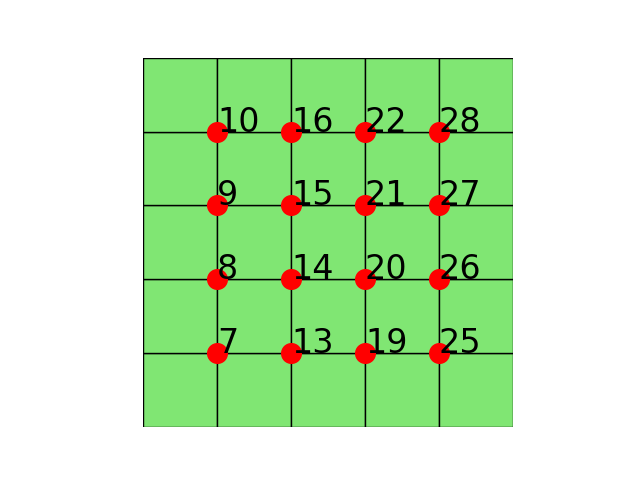
\includegraphics[scale=0.7]{./figures/1.png}
\caption{}
\end{figure}
两边取点$n_1=n_2=4$时,$h_1=h_2=\frac{1}{n+1}$利用五点中心近似
$$\vartriangle u(x)\approx\frac{1}{h^2}[u(x_1+h,x_2)+u(x_1-h,x_2)+u(x_1,x_2+h)+u(x_1,x_2-h)-4u(x_1,x_2)]$$
得
$$A=\frac{1}{h^2}\begin{bmatrix}
B & {-I}\\
-I & B & {-I}\\
 & {-I} & B
\end{bmatrix}$$
其中
$$B=\begin{bmatrix}
4 & {-1}\\
-1 & 4 & {-1}\\
  & {-1} & 4 & {-1}\\
  & & {-1} & 4
 \end{bmatrix}$$





















































%\newtheorem{thm}{定理}
%\begin{thm}

%\end{thm}



































%函数$y(x)$的变分定义为$\delta y=y_1(x)-y(x)$,其中$y_1(x)$是“靠近”$y(x)$的一个函数,即$\delta y$是同一自变量$x$处相邻函数的函数值之差。

%注意:

%$(\delta y)'=y'_1(x)-y'(x)=\delta y'$

%$(\delta y)^n=\delta y^n $
%\subsection{泛函的变分}
%定义泛函$J[y(x)]=\int_{a}^{b} f(x,y,y')\mathrm{d}x$,则增量$\bigtriangleup J=\int_{a}^{b}[f(x,y+\delta y,y'+\delta y')-f(x,y,y')]\mathrm{d}x=\int_{a}^{b}[\frac{\partial f}{\partial y}\delta y + \frac{\partial f}{\partial y'}\delta y'+\frac{1}{2}\frac{\partial^2 f}{\partial^2 y}(\delta y)^2+\frac{\partial^2 f}{\partial y\,\partial y'}\delta y\delta y'+\frac{1}{2}\frac{\partial^2 f}{\partial y'^2}(\partial y')^2+\cdots]\mathrm{d}x$

%舍弃掉$\delta y$和$\delta y'$二次项及以上的高次项,得到关于$\delta y$和$\delta y'$一次项的和,称为$J[y(X)]=\int_{a}^{b} f(x,y,y')\mathrm{d}x$的一阶变分,简称为泛函的变分,即$\delta J=\int_{a}^{b}(\frac{\partial f}{\partial y}\delta y + \frac{\partial f}{\partial y'}\delta y')\mathrm{d}x$。
%\subsection{泛函变分的基本运算法则}
%泛函变分运算法则与微分运算法则基本相同

%$(\delta F_1 +F_2)=\delta F_1 +\delta F_2$

%$(\delta F)^n=nF^n-1\delta F$

%$(\delta F_1 \cdot F_2)=F_2\delta F_1+F_1\delta F_2$

%$(\delta (\frac{F_1}{F_2})=\frac{1}{F^2_2}(F_2\delta F_1-F_1\delta F_2)$

%$\delta\int_{a}^{b}F\mathrm{d}x=\int_{a}^{b}\delta F\mathrm{d}x$







%如果将泛函取极值时的函数定义为$y(x)$,并且定义与函数$y(x)$相靠近的函数为$y(x,\varepsilon)$,记为$y(x,\varepsilon)=y(x)+\varepsilon\eta(x)$,$\varepsilon$是一个参数。
%函数$y(x)$的变分定义为$\delta y=\eta(x)\mathrm{d}\varepsilon$,由此可得$\delta y'=\eta ^\prime(x)\mathrm{d}\varepsilon$
%定义泛函$J[y(X)]=\int_{a}^{b} F(x,y,y')\mathrm{d}x$的变分为$\delta J=\int_{a}^{b}(\frac{\partial F}{\partial y}\delta y + \frac{\partial F}{\partial y'}\delta y')\mathrm{d}x$。

%\subsection{泛函变分举例}
%计算泛函$J[y(x)]=\int_{-1}^{1} (y'e^7 +xy^2)\mathrm{d}x$的变分


%$\delta J[y(x)]=\delta\int_{-1}^{1}(y'e^7+xy^2)\mathrm{d}x=\int_{-1}^{1}(2xy\delta y+e^7\delta y')\mathrm{d}x=\int_{-1}^{1}(2xy\delta y)\mathrm{d}x+\int_{-1}^{1}e^7\mathrm{d}\delta y=\int_{-1}^{1}(2xy\delta y)\mathrm{d}x
%$,最后一步利用上边界上函数变分为0。






%\begin{equation}
%-\nabla \cdot (\beta\nabla u) = f(x,y),\,\ (x,y)\in \Omega
%\end{equation}
%Dilichlet 边界条件

%\begin{equation}
%u(x,y) = g(x,y),\,\ (x,y)\in \partial \Omega
%\end{equation}
%\subsection{符号}
%\begin{tabular}{ |l|l| }   
%\hline   
%\multicolumn{2}{|c|}{符号说明} \\   
%\hline
%符号 & 含义\\
%\hline
%$\Omega$ & 二维长方形区域 \\
%\hline
%$nx$ & $x$ 方向剖分的段数 \\
%\hline
%$ny$ & $y$ 方向剖分的段数 \\
%\hline
%$hx$ &  $x$ 方向每段的长度\\
%\hline
%$hy$ &  $y$ 方向每段的长度 \\
%\hline
%$\mu$ & $the \,\ viscosity \,\ coefficient$ \\
%\hline
%$k$ & $the \,\ permeability \,\ tensor$ \\
%\hline 
%$NC$ & 代表 $cell$ 的个数 \\
%\hline
%$NE$ & 代表总的 $edge$ 的个数 \\
%\hline
%\end{tabular}

%\section{欧拉—拉格朗日方程}
%欧拉—拉格朗日方程是泛函极值问题的必要条件,假设$J[y(x)]$的极值问题的解为$y=y(x)$,现在推导这个解所满足的微分方程。

%$\delta J=\int_{a}^{b}(\frac{\partial f}{\partial y}\delta y + \frac{\partial f}{\partial y'}\delta y')\mathrm{d}x=0$,将第二项分部积分得到$\int_{a}^{b}(\frac{\partial f}{\partial y'}\delta y')\mathrm{d}x=\int_{a}^{b}\frac{\partial f}{\partial y'}\mathrm{d}\delta y$,因为$\delta y(a)=0$,$\delta y(b)=0$,所以$\int_{a}^{b}(\frac{\partial f}{\partial y'}\delta y')\mathrm{d}x=-\int_{a}^{b}\delta y\mathrm{d}\frac{\partial f}{\partial y'}$,因此$\delta J=\int_{a}^{b}\frac{\partial f}{\partial y}\delta y\mathrm{d}x-\int_{a}^{b}\delta y\mathrm{d}\frac{\partial f}{\partial y'}=\int_{a}^{b}(\frac{\partial f}{\partial y}-\frac{\mathrm{d}\frac{\partial f}{\partial y'}}{\mathrm{d}x})\delta y\mathrm{d}x=0$,因为对于任何函数$\delta y$都成立,故$\frac{\partial f}{\partial y}-\frac{\mathrm{d}\frac{\partial f}{\partial y'}}{\mathrm{d}x}=0$,这就是欧拉—拉格朗日方程。
%\begin{equation*}
%\begin{cases}
%\begin{aligned}
%\frac{\mu}{k}\mathbf{u} + \nabla p & = 0 \quad in \,\ \Omega = (0,1)\times (0,1) \\
%\nabla \cdot \mathbf{u} & = f \quad in \,\ \Omega \\
%\mathbf {u} & = 0 \quad on \,\ \partial \Omega
%\end{aligned}
%\end{cases}
%\end{equation*}

%且有 \\
%\begin{equation*}
%\int_{\Omega}f dxdy = 0
%\end{equation*}

%记 $u$ 为 $\mathbf{u}$ 在 $x$ 方向的分量,$v$ 为 $\mathbf{u}$ 在 $y$ 方向的分量,则有 \\

%\begin{equation*}
%\begin{cases}
%\begin{aligned}
%\frac{\mu}{k}\cdot u + \partial_x p & = 0 \quad (1) \\
%\frac{\mu}{k}\cdot v + \partial_y p & = 0 \quad (2) \\
%\partial_x u + \partial_y v & = f \quad (3)
%\end{aligned}
%\end{cases}
%\end{equation*}

%\section{离散后组装矩阵}
%利用一阶向前差分把方程变成差分方程,现在从 $edge$ 和 $cell$ 的角度考虑模型。 \\

%对于 $(1)$, 从内部纵向 $edge$ 的角度考虑:
%我们需要找到内部纵向 $edge$ 所对应的左手边的 $cell$ 和右手边的 $cell$. 左右两边的$cell$ 所对应的 $p$ 分别记为 $p_{l}$、$p_{r}$.$u$ 为 $edge$ 的中点,记为 $u_m$。按照 $mesh$ 里的编号规则排序。\\

%则每条内部边上所对应的差分方程为:

%\begin{equation*}
%\frac{\mu}{k} \cdot u_m + \frac{p_r - p_l}{hx} = 0
%\end{equation*}

%对于 $(2)$,从内部横向 $edge$ 的角度考虑:
%我们需要找到内部横向 $edge$ 所对应的左手边的 $cell$ 和右手边的 $cell$. $cell$ 所对应的 $p$ 与 $(1)$ 中的相同。$v$ 为 $edge$ 的中点,记为 $v_m$。\\

%则每条内部边上所对应的差分方程为:\\

%\begin{equation*}
%\frac{\mu}{k} \cdot v_m + \frac{p_l - p_r}{hy} = 0
%\end{equation*}

%对于 $(3)$, 从 $cell$ 的角度考虑:
%由于单元是四边形单元,我们记单元所对应边的局部编号为[0,1,2,3](StructureQuadMesh.py 里的网格),第 $i$ 个单元所对应的边记为 $e_{i,0},e_{i,1},e_{i,2},e_{i,3}$。\\

%则 $(3)$ 式第 $i$ 个单元所对应的差分方程为:\\

%\begin{equation*}
%\frac{u_{e_{i,1}} - u_{e_{i,3}}}{hx} + \frac{v_{e_{i,2}} - v_{e_{i,0}}}{hy} = f_i
%\end{equation*}

%我们需要生成一个 $(NE+NC)\times(NE+NC)$的系数矩阵,把它看成分块矩阵
%\begin{equation*}
%\begin{pmatrix}
% A_{1,1} & A_{1,2} \\
%A_{2,1} & A_{2,2}
%\end{pmatrix}
%\end{equation*}

%其中 \\

%\begin{equation*}
%\begin{aligned}
%A_{1,1} : NE\times NE \\
%A_{1,2} : NE\times NC \\
%A_{2,1} : NC\times NE \\
%A_{2,2} : NC\times NC
%\end{aligned}
%\end{equation*}

%$A_{1,1}$ 对应的是 $(1),(2)$ 两式的第一项,即含有 $u,v$ 的项,$A_12$ 对应的是 $(1),(2)$ 两式的第二项。

%\newpage
%\nocite{*}
%\bibliography{ref}
\end{document}

